\documentclass[12pt]{article}
\usepackage{latexblog}

% ============================================================
% Blog Metadata
% ============================================================
\blogtitle{Hadoop(1)：Hadoop是什么}
\blogdate{2021-09-28}
\blogtags{Hadoop, 大数据}
\bloglang{zh}
\blogsummary{}

\begin{document}
\makeblogtitle

Apache Hadoop是一个分布式的大数据处理框架，在2008年击败超级计算机，成为最快排序1TB数据的系统，用时209秒。

\section{Hadoop发展历史}\label{hadoopux53d1ux5c55ux5386ux53f2}

\begin{itemize}
\tightlist
\item
  2002年，Doug Cutting 和Mike Cafarella在Lucene的基础之上开发了Nutch，一款开源搜索引擎
\item
  2003年，Google发表了GFS(Google File System)的论文，这是其为存储海量搜索数据而设计的文件系统
\item
  2004年，Doug基于GFS论文实现了分布式文件存储系统，命名为NDFS；同年Google发表了MapReduce编程模型，用于大规模数据的并行分析计算
\item
  2005年，Doug基于MapReduce，在Nutch中也实现了该功能
\item
  2006年，Nutch成为Apache的项目并改名为Hadoop，当时还只能在20\textasciitilde40个节点上运行。Doug也加入Yahoo并将Hadoop扩展到可以在上千节点的集群上运行
\item
  2007年，Yahoo开始在1000个节点的集群上使用Hadoop
\item
  2008年，Hadoop成为Apache的顶级项目，许多其他公司例如Facebook等也开始使用Hadoop
\end{itemize}

总体来讲，Hadoop基本上是跟着Google的步伐来的：

\begin{itemize}
\tightlist
\item
  GFS → HDFS
\item
  MapReduce → MapReduce
\item
  BigTable → HBase
\end{itemize}

\section{Hadoop基础概念}\label{hadoopux57faux7840ux6982ux5ff5}

\subsection{HDFS}\label{hdfs}

\begin{figure}
\centering
\pandocbounded{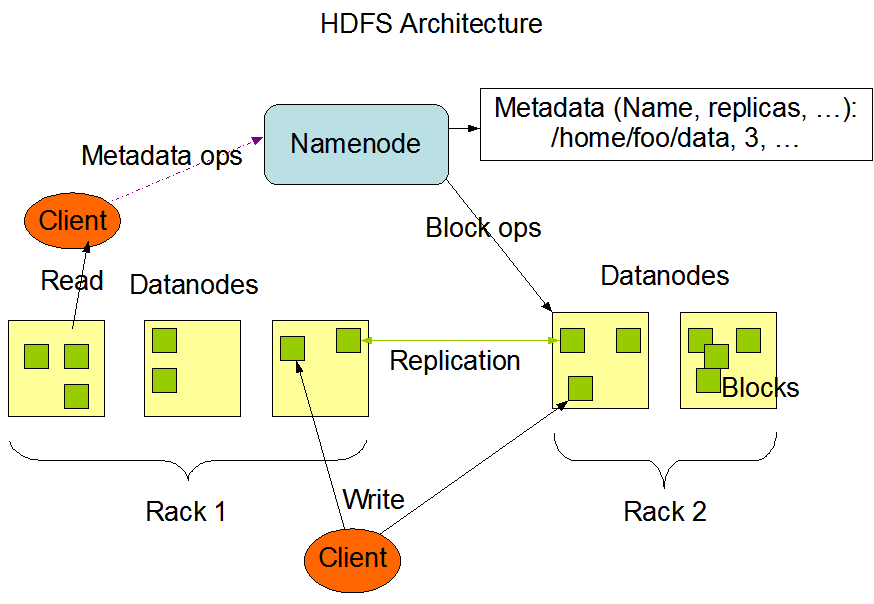
\includegraphics[keepaspectratio,alt={HDFS Architecture}]{images/hdfs-architecture.png}}
\caption{HDFS Architecture}
\end{figure}

HDFS是一个主从架构，一个HDFS集群包含一个NameNode和多个DataNode。HDFS暴露文件系统命名空间，允许用户以文件的方式存储；在其内部一个文件会被切分成一个或者多个块存储在一系列的数据节点上。

\begin{itemize}
\tightlist
\item
  NameNode: 主节点，管理集群的文件命名空间、元数据等，并控制客户端访问。真正存储的数据是不会经过NameNode的。
\item
  DataNode: 数据节点，通常每个机器上部署一个该节点来管理存储，根据NameNode的调度来执行块的创建、删除、复制等操作
\end{itemize}

\subsection{MapReduce}\label{mapreduce}

MapReduce是一个并行计算的编程模型，最早由谷歌提出，用来处理其海量的网页数据，为搜索引擎服务。MapReduce能够通过集群的方式进行水平扩展，可以利用廉价的计算机进行计算，处理海量的数据。MapReduce一般分为三步：

\begin{itemize}
\tightlist
\item
  \textbf{Map}: 每一个计算节点对本地数据应用\texttt{map}方法，将结果输出到临时存储。
\item
  \textbf{Shuffle}: 计算节点对上一步的输出进行重新分布，保证同一个key下的数据都在同一个节点之上
\item
  \textbf{Reduce}: 并行的处理每一个key的数据
\end{itemize}

如下是一个统计单次出现频次的MapReduce的典型过程：

\begin{figure}
\centering
\pandocbounded{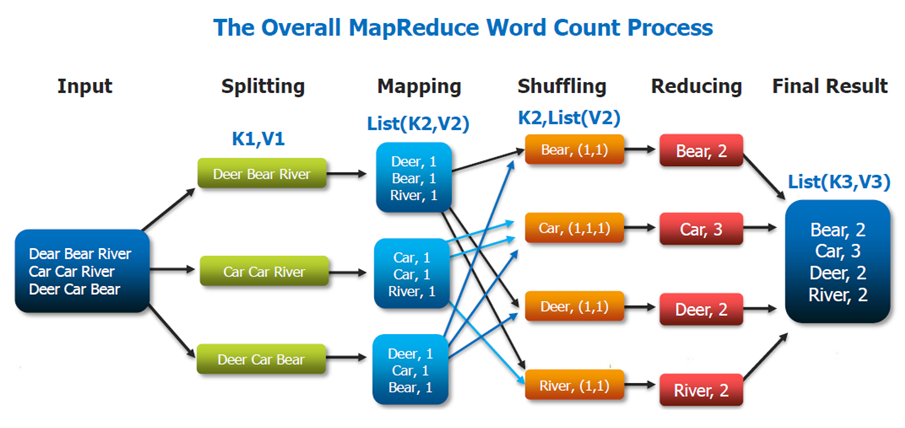
\includegraphics[keepaspectratio,alt={Word Count}]{images/Word-count.png}}
\caption{Word Count}
\end{figure}

\section{Hadoop生态}\label{hadoopux751fux6001}

除了Hadoop本身之外，还有不少框架是围绕着Hadoop而服务的，主要包括有以下：

\begin{itemize}
\tightlist
\item
  \textbf{Apache Flume}: 分布式的日志收集/聚合系统
\item
  \textbf{Apache Hadoop YARN}: Hadoop的资源管理/任务调度框架
\item
  \textbf{Apache HBase}: 分布式大数据NoSQL数据库，基于Bigtable和HDFS
\item
  \textbf{Apache Hive}: 基于Hadoop的数仓查询工具，可以通过SQL来进行读写
\item
  \textbf{Presto}: 分布式大数据SQL查询引擎
\item
  \textbf{Apache Oozie}: Hadoop的工作流调度系统
\item
  \textbf{Apache Pig}: 基于Hadoop的大规模数据分析平台，提供的SQL-LIKE语言叫Pig Latin，把数据分析请求转换为一系列经过优化处理的MapReduce运算
\item
  \textbf{Apache Sqoop}: 一个在Hadoop和传统关系型数据库之间数据传输的工具
\item
  \textbf{Apache Zookeeper}: 分布式协调系统
\item
  \textbf{Apache Impala}: 为Hadoop提供的一个SQL查询引擎
\item
  \textbf{Apache Solr}: 基于Apache Lucene的搜索引擎
\item
  \textbf{Apache Spark}: 一个大数据分析引擎
\item
  \textbf{Apache Storm}: 一个分布式实时计算系统
\item
  \ldots{}
\end{itemize}

参考:

\begin{itemize}
\tightlist
\item
  \href{https://data-flair.training/blogs/hadoop-history/}{History of Hadoop -- The complete evolution of Hadoop Ecosytem}
\end{itemize}


\end{document}
